% Options for packages loaded elsewhere
\PassOptionsToPackage{unicode}{hyperref}
\PassOptionsToPackage{hyphens}{url}
%
\documentclass[
]{article}
\usepackage{amsmath,amssymb}
\usepackage{lmodern}
\usepackage{ifxetex,ifluatex}
\ifnum 0\ifxetex 1\fi\ifluatex 1\fi=0 % if pdftex
  \usepackage[T1]{fontenc}
  \usepackage[utf8]{inputenc}
  \usepackage{textcomp} % provide euro and other symbols
\else % if luatex or xetex
  \usepackage{unicode-math}
  \defaultfontfeatures{Scale=MatchLowercase}
  \defaultfontfeatures[\rmfamily]{Ligatures=TeX,Scale=1}
\fi
% Use upquote if available, for straight quotes in verbatim environments
\IfFileExists{upquote.sty}{\usepackage{upquote}}{}
\IfFileExists{microtype.sty}{% use microtype if available
  \usepackage[]{microtype}
  \UseMicrotypeSet[protrusion]{basicmath} % disable protrusion for tt fonts
}{}
\makeatletter
\@ifundefined{KOMAClassName}{% if non-KOMA class
  \IfFileExists{parskip.sty}{%
    \usepackage{parskip}
  }{% else
    \setlength{\parindent}{0pt}
    \setlength{\parskip}{6pt plus 2pt minus 1pt}}
}{% if KOMA class
  \KOMAoptions{parskip=half}}
\makeatother
\usepackage{xcolor}
\IfFileExists{xurl.sty}{\usepackage{xurl}}{} % add URL line breaks if available
\IfFileExists{bookmark.sty}{\usepackage{bookmark}}{\usepackage{hyperref}}
\hypersetup{
  pdftitle={KBH\_94\_23\_DE\_5\_all\_pyx\_lines},
  hidelinks,
  pdfcreator={LaTeX via pandoc}}
\urlstyle{same} % disable monospaced font for URLs
\usepackage[margin=1in]{geometry}
\usepackage{color}
\usepackage{fancyvrb}
\newcommand{\VerbBar}{|}
\newcommand{\VERB}{\Verb[commandchars=\\\{\}]}
\DefineVerbatimEnvironment{Highlighting}{Verbatim}{commandchars=\\\{\}}
% Add ',fontsize=\small' for more characters per line
\usepackage{framed}
\definecolor{shadecolor}{RGB}{248,248,248}
\newenvironment{Shaded}{\begin{snugshade}}{\end{snugshade}}
\newcommand{\AlertTok}[1]{\textcolor[rgb]{0.94,0.16,0.16}{#1}}
\newcommand{\AnnotationTok}[1]{\textcolor[rgb]{0.56,0.35,0.01}{\textbf{\textit{#1}}}}
\newcommand{\AttributeTok}[1]{\textcolor[rgb]{0.77,0.63,0.00}{#1}}
\newcommand{\BaseNTok}[1]{\textcolor[rgb]{0.00,0.00,0.81}{#1}}
\newcommand{\BuiltInTok}[1]{#1}
\newcommand{\CharTok}[1]{\textcolor[rgb]{0.31,0.60,0.02}{#1}}
\newcommand{\CommentTok}[1]{\textcolor[rgb]{0.56,0.35,0.01}{\textit{#1}}}
\newcommand{\CommentVarTok}[1]{\textcolor[rgb]{0.56,0.35,0.01}{\textbf{\textit{#1}}}}
\newcommand{\ConstantTok}[1]{\textcolor[rgb]{0.00,0.00,0.00}{#1}}
\newcommand{\ControlFlowTok}[1]{\textcolor[rgb]{0.13,0.29,0.53}{\textbf{#1}}}
\newcommand{\DataTypeTok}[1]{\textcolor[rgb]{0.13,0.29,0.53}{#1}}
\newcommand{\DecValTok}[1]{\textcolor[rgb]{0.00,0.00,0.81}{#1}}
\newcommand{\DocumentationTok}[1]{\textcolor[rgb]{0.56,0.35,0.01}{\textbf{\textit{#1}}}}
\newcommand{\ErrorTok}[1]{\textcolor[rgb]{0.64,0.00,0.00}{\textbf{#1}}}
\newcommand{\ExtensionTok}[1]{#1}
\newcommand{\FloatTok}[1]{\textcolor[rgb]{0.00,0.00,0.81}{#1}}
\newcommand{\FunctionTok}[1]{\textcolor[rgb]{0.00,0.00,0.00}{#1}}
\newcommand{\ImportTok}[1]{#1}
\newcommand{\InformationTok}[1]{\textcolor[rgb]{0.56,0.35,0.01}{\textbf{\textit{#1}}}}
\newcommand{\KeywordTok}[1]{\textcolor[rgb]{0.13,0.29,0.53}{\textbf{#1}}}
\newcommand{\NormalTok}[1]{#1}
\newcommand{\OperatorTok}[1]{\textcolor[rgb]{0.81,0.36,0.00}{\textbf{#1}}}
\newcommand{\OtherTok}[1]{\textcolor[rgb]{0.56,0.35,0.01}{#1}}
\newcommand{\PreprocessorTok}[1]{\textcolor[rgb]{0.56,0.35,0.01}{\textit{#1}}}
\newcommand{\RegionMarkerTok}[1]{#1}
\newcommand{\SpecialCharTok}[1]{\textcolor[rgb]{0.00,0.00,0.00}{#1}}
\newcommand{\SpecialStringTok}[1]{\textcolor[rgb]{0.31,0.60,0.02}{#1}}
\newcommand{\StringTok}[1]{\textcolor[rgb]{0.31,0.60,0.02}{#1}}
\newcommand{\VariableTok}[1]{\textcolor[rgb]{0.00,0.00,0.00}{#1}}
\newcommand{\VerbatimStringTok}[1]{\textcolor[rgb]{0.31,0.60,0.02}{#1}}
\newcommand{\WarningTok}[1]{\textcolor[rgb]{0.56,0.35,0.01}{\textbf{\textit{#1}}}}
\usepackage{graphicx}
\makeatletter
\def\maxwidth{\ifdim\Gin@nat@width>\linewidth\linewidth\else\Gin@nat@width\fi}
\def\maxheight{\ifdim\Gin@nat@height>\textheight\textheight\else\Gin@nat@height\fi}
\makeatother
% Scale images if necessary, so that they will not overflow the page
% margins by default, and it is still possible to overwrite the defaults
% using explicit options in \includegraphics[width, height, ...]{}
\setkeys{Gin}{width=\maxwidth,height=\maxheight,keepaspectratio}
% Set default figure placement to htbp
\makeatletter
\def\fps@figure{htbp}
\makeatother
\setlength{\emergencystretch}{3em} % prevent overfull lines
\providecommand{\tightlist}{%
  \setlength{\itemsep}{0pt}\setlength{\parskip}{0pt}}
\setcounter{secnumdepth}{-\maxdimen} % remove section numbering
\usepackage{booktabs}
\usepackage{longtable}
\usepackage{array}
\usepackage{multirow}
\usepackage{wrapfig}
\usepackage{float}
\usepackage{colortbl}
\usepackage{pdflscape}
\usepackage{tabu}
\usepackage{threeparttable}
\usepackage{threeparttablex}
\usepackage[normalem]{ulem}
\usepackage{makecell}
\usepackage{xcolor}
\ifluatex
  \usepackage{selnolig}  % disable illegal ligatures
\fi

\title{KBH\_94\_23\_DE\_5\_all\_pyx\_lines}
\author{}
\date{\vspace{-2.5em}}

\begin{document}
\maketitle

\hypertarget{both-cpx-and-opx-are-included}{%
\subsection{Both CPX and OPX are
included}\label{both-cpx-and-opx-are-included}}

Line 1 OPX Line 3 CPX Line 4 OPX Line OPX Line 5 OPX/CPX/OPX

\hypertarget{line-5}{%
\subsubsection{Line 5}\label{line-5}}

is a tiny CPX inside of a larger OPX

\begin{figure}
\centering
\includegraphics{M5_DE_KBH_23.JPG}
\caption{alt text}
\end{figure}

\#Bring in the CSV

\hypertarget{section}{%
\subsection{}\label{section}}

Not working \%\textgreater\% filter(!is.na(phos\_ox))

\hypertarget{ternary-of-both-opx-and-cpx}{%
\section{Ternary of both OPX and
CPX:}\label{ternary-of-both-opx-and-cpx}}

\begin{Shaded}
\begin{Highlighting}[]
\NormalTok{MgO\_num }\OtherTok{\textless{}{-}} \FunctionTok{mutate}\NormalTok{(M5\_DE\_all\_pyx\_KBH\_94\_23, }\AttributeTok{mg\_dat =}\NormalTok{ MgO}\SpecialCharTok{/}\FloatTok{40.304}\NormalTok{,}
                  \AttributeTok{fe\_dat =}\NormalTok{ FeO}\SpecialCharTok{/}\FloatTok{71.844}\NormalTok{,}
                  \AttributeTok{ca\_dat =}\NormalTok{ CaO}\SpecialCharTok{/}\FloatTok{56.077}\NormalTok{,}
                  \AttributeTok{Mg =}\NormalTok{ (mg\_dat}\SpecialCharTok{/}\NormalTok{(mg\_dat}\SpecialCharTok{+}\NormalTok{fe\_dat}\SpecialCharTok{+}\NormalTok{ca\_dat))}\SpecialCharTok{*}\DecValTok{100}\NormalTok{,}
                  \AttributeTok{Fe =}\NormalTok{ (fe\_dat}\SpecialCharTok{/}\NormalTok{(mg\_dat}\SpecialCharTok{+}\NormalTok{fe\_dat}\SpecialCharTok{+}\NormalTok{ca\_dat))}\SpecialCharTok{*}\DecValTok{100}\NormalTok{,}
                  \AttributeTok{Ca =}\NormalTok{ (ca\_dat}\SpecialCharTok{/}\NormalTok{(mg\_dat}\SpecialCharTok{+}\NormalTok{fe\_dat}\SpecialCharTok{+}\NormalTok{ca\_dat))}\SpecialCharTok{*}\DecValTok{100}
\NormalTok{                  )}
                  
\NormalTok{MgO\_num }\SpecialCharTok{\%\textgreater{}\%} 
  \FunctionTok{kbl}\NormalTok{() }\SpecialCharTok{\%\textgreater{}\%} 
  \FunctionTok{kable\_styling}\NormalTok{(}\AttributeTok{bootstrap\_options =} \FunctionTok{c}\NormalTok{(}\StringTok{"striped"}\NormalTok{, }\StringTok{"hover"}\NormalTok{, }\StringTok{"condensed"}\NormalTok{, }\StringTok{"responsive"}\NormalTok{))}
\end{Highlighting}
\end{Shaded}

\begin{table}
\centering
\begin{tabular}[t]{l|r|r|r|r|r|r|r|r|r|r|r|r|r|r|r|r|r|r}
\hline
OPX & P2O5 & SiO2 & TiO2 & Al2O3 & Cr2O3 & MgO & CaO & MnO & FeO & NiO & Na2O & K2O & mg\_dat & fe\_dat & ca\_dat & Mg & Fe & Ca\\
\hline
1.1 & 0 & 52.856 & 0.241 & 5.803 & 0.359 & 30.472 & 1.166 & 0.138 & 8.740 & 0 & 0.134 & 0.009 & 0.7560540 & 0.1216525 & 0.0207928 & 84.14631 & 13.539518 & 2.314174\\
\hline
1.2 & 0 & 53.478 & 0.222 & 5.786 & 0.401 & 30.686 & 1.172 & 0.184 & 8.753 & 0 & 0.122 & 0.003 & 0.7613636 & 0.1218334 & 0.0208998 & 84.21262 & 13.475704 & 2.311681\\
\hline
1.3 & 0 & 53.457 & 0.226 & 5.678 & 0.403 & 30.807 & 1.133 & 0.182 & 8.847 & 0 & 0.142 & 0.000 & 0.7643658 & 0.1231418 & 0.0202044 & 84.20797 & 13.566176 & 2.225856\\
\hline
1.4 & 0 & 53.029 & 0.223 & 5.569 & 0.409 & 30.364 & 1.132 & 0.178 & 8.758 & 0 & 0.123 & 0.001 & 0.7533744 & 0.1219030 & 0.0201865 & 84.13230 & 13.613392 & 2.254310\\
\hline
1.5 & 0 & 53.688 & 0.190 & 5.548 & 0.410 & 30.993 & 1.133 & 0.188 & 8.806 & 0 & 0.140 & 0.000 & 0.7689807 & 0.1225711 & 0.0202044 & 84.34061 & 13.443410 & 2.215983\\
\hline
1.6 & 0 & 53.717 & 0.188 & 5.466 & 0.403 & 30.922 & 1.131 & 0.158 & 8.783 & 0 & 0.114 & 0.006 & 0.7672191 & 0.1222510 & 0.0201687 & 84.34327 & 13.439509 & 2.217220\\
\hline
1.7 & 0 & 53.728 & 0.218 & 5.446 & 0.437 & 30.982 & 1.094 & 0.166 & 8.770 & 0 & 0.127 & 0.006 & 0.7687078 & 0.1220700 & 0.0195089 & 84.44678 & 13.410065 & 2.143159\\
\hline
1.8 & 0 & 53.836 & 0.203 & 5.507 & 0.407 & 30.894 & 1.144 & 0.193 & 8.755 & 0 & 0.120 & 0.000 & 0.7665244 & 0.1218613 & 0.0204005 & 84.34596 & 13.409233 & 2.244810\\
\hline
1.9 & 0 & 53.026 & 0.216 & 5.347 & 0.426 & 30.581 & 1.133 & 0.160 & 8.813 & 0 & 0.120 & 0.000 & 0.7587584 & 0.1226686 & 0.0202044 & 84.15395 & 13.605179 & 2.240867\\
\hline
1.1\_0 & 0 & 53.834 & 0.205 & 5.523 & 0.414 & 30.857 & 1.136 & 0.188 & 8.671 & 0 & 0.125 & 0.003 & 0.7656064 & 0.1206921 & 0.0202579 & 84.45216 & 13.313244 & 2.234595\\
\hline
1.11 & 0 & 53.688 & 0.185 & 5.563 & 0.438 & 30.974 & 1.197 & 0.183 & 8.762 & 0 & 0.150 & 0.010 & 0.7685093 & 0.1219587 & 0.0213456 & 84.28359 & 13.375396 & 2.341010\\
\hline
1.12 & 0 & 53.498 & 0.235 & 5.547 & 0.438 & 30.689 & 1.150 & 0.181 & 8.800 & 0 & 0.122 & 0.000 & 0.7614381 & 0.1224876 & 0.0205075 & 84.18953 & 13.543025 & 2.267444\\
\hline
1.13 & 0 & 53.582 & 0.224 & 5.635 & 0.409 & 30.970 & 1.177 & 0.183 & 8.824 & 0 & 0.154 & 0.000 & 0.7684101 & 0.1228217 & 0.0209890 & 84.23510 & 13.464029 & 2.300868\\
\hline
1.14 & 0 & 53.930 & 0.258 & 5.867 & 0.444 & 31.142 & 1.197 & 0.189 & 8.780 & 0 & 0.147 & 0.002 & 0.7726776 & 0.1222092 & 0.0213456 & 84.33205 & 13.338233 & 2.329720\\
\hline
3.1 & 0 & 50.280 & 0.768 & 7.590 & 0.792 & 15.494 & 18.796 & 0.132 & 4.841 & 0 & 1.414 & 0.005 & 0.3844283 & 0.0673821 & 0.3351820 & 48.84778 & 8.561976 & 42.590242\\
\hline
3.2 & 0 & 50.846 & 0.691 & 7.449 & 0.828 & 15.651 & 18.924 & 0.133 & 4.720 & 0 & 1.417 & 0.013 & 0.3883237 & 0.0656979 & 0.3374646 & 49.06260 & 8.300574 & 42.636822\\
\hline
3.3 & 0 & 50.933 & 0.661 & 7.485 & 0.844 & 15.916 & 18.842 & 0.122 & 4.710 & 0 & 1.417 & 0.009 & 0.3948988 & 0.0655587 & 0.3360023 & 49.58176 & 8.231265 & 42.186975\\
\hline
3.4 & 0 & 50.851 & 0.622 & 7.432 & 0.842 & 15.792 & 18.879 & 0.137 & 4.602 & 0 & 1.428 & 0.013 & 0.3918222 & 0.0640555 & 0.3366621 & 49.43880 & 8.082302 & 42.478893\\
\hline
3.5 & 0 & 50.672 & 0.606 & 7.489 & 0.861 & 15.741 & 18.878 & 0.112 & 4.690 & 0 & 1.411 & 0.012 & 0.3905568 & 0.0652803 & 0.3366443 & 49.28277 & 8.237459 & 42.479770\\
\hline
3.6 & 0 & 51.316 & 0.579 & 7.524 & 0.856 & 15.952 & 18.725 & 0.105 & 4.583 & 0 & 1.421 & 0.000 & 0.3957920 & 0.0637910 & 0.3339159 & 49.87934 & 8.039204 & 42.081456\\
\hline
3.7 & 0 & 50.778 & 0.562 & 7.525 & 0.856 & 15.826 & 18.827 & 0.122 & 4.583 & 0 & 1.421 & 0.009 & 0.3926657 & 0.0637910 & 0.3357348 & 49.56702 & 8.052471 & 42.380508\\
\hline
3.8 & 0 & 50.301 & 0.556 & 7.407 & 0.886 & 15.573 & 18.786 & 0.115 & 4.631 & 0 & 1.343 & 0.004 & 0.3863884 & 0.0644591 & 0.3350037 & 49.16814 & 8.202457 & 42.629400\\
\hline
3.9 & 0 & 50.890 & 0.611 & 7.434 & 0.867 & 15.790 & 18.995 & 0.140 & 4.601 & 0 & 1.429 & 0.000 & 0.3917725 & 0.0640415 & 0.3387307 & 49.30780 & 8.060155 & 42.632045\\
\hline
3.1\_0 & 0 & 50.838 & 0.581 & 7.503 & 0.843 & 15.678 & 18.837 & 0.113 & 4.586 & 0 & 1.418 & 0.006 & 0.3889936 & 0.0638327 & 0.3359131 & 49.31839 & 8.093008 & 42.588600\\
\hline
3.11 & 0 & 52.314 & 0.551 & 7.880 & 0.745 & 16.686 & 17.331 & 0.115 & 4.454 & 0 & 1.492 & 0.000 & 0.4140036 & 0.0619954 & 0.3090572 & 52.73553 & 7.896942 & 39.367524\\
\hline
3.12 & 0 & 52.908 & 0.633 & 7.932 & 0.828 & 16.984 & 18.942 & 0.127 & 4.693 & 0 & 1.565 & 0.001 & 0.4213974 & 0.0653221 & 0.3377855 & 51.10914 & 7.922582 & 40.968283\\
\hline
3.13 & 0 & 55.104 & 0.647 & 8.541 & 0.807 & 18.081 & 18.938 & 0.119 & 4.636 & 0 & 1.832 & 0.009 & 0.4486155 & 0.0645287 & 0.3377142 & 52.72505 & 7.583953 & 39.690999\\
\hline
3.14 & 0 & 50.560 & 0.669 & 7.394 & 0.798 & 15.571 & 18.832 & 0.133 & 4.839 & 0 & 1.396 & 0.009 & 0.3863388 & 0.0673543 & 0.3358240 & 48.93356 & 8.531072 & 42.535365\\
\hline
3.15 & 0 & 50.575 & 0.765 & 6.659 & 0.785 & 16.227 & 19.999 & 0.115 & 4.725 & 0 & 0.876 & 0.002 & 0.4026151 & 0.0657675 & 0.3566346 & 48.80081 & 7.971651 & 43.227536\\
\hline
4.1 & 0 & 48.348 & 0.402 & 5.592 & 0.068 & 36.200 & 0.911 & 0.208 & 13.173 & 0 & 0.027 & 0.024 & 0.8981739 & 0.1833556 & 0.0162455 & 81.81767 & 16.702476 & 1.479859\\
\hline
4.2 & 0 & 53.648 & 0.242 & 5.827 & 0.350 & 30.748 & 1.204 & 0.163 & 8.860 & 0 & 0.134 & 0.003 & 0.7629019 & 0.1233228 & 0.0214705 & 84.04825 & 13.586362 & 2.365384\\
\hline
4.3 & 0 & 52.614 & 0.255 & 5.898 & 0.339 & 29.886 & 1.307 & 0.177 & 8.700 & 0 & 0.158 & 0.021 & 0.7415145 & 0.1210957 & 0.0233072 & 83.70018 & 13.668961 & 2.630859\\
\hline
4.4 & 0 & 53.524 & 0.236 & 5.799 & 0.363 & 30.898 & 1.214 & 0.218 & 8.914 & 0 & 0.135 & 0.000 & 0.7666237 & 0.1240744 & 0.0216488 & 84.02765 & 13.599475 & 2.372870\\
\hline
4.5 & 0 & 53.463 & 0.247 & 5.798 & 0.367 & 30.512 & 1.162 & 0.170 & 8.837 & 0 & 0.137 & 0.000 & 0.7570464 & 0.1230026 & 0.0207215 & 84.04431 & 13.655266 & 2.300420\\
\hline
4.6 & 0 & 53.693 & 0.283 & 5.824 & 0.381 & 30.791 & 1.186 & 0.190 & 8.819 & 0 & 0.142 & 0.000 & 0.7639688 & 0.1227521 & 0.0211495 & 84.14955 & 13.520881 & 2.329572\\
\hline
4.7 & 0 & 53.631 & 0.246 & 5.775 & 0.364 & 30.590 & 1.158 & 0.191 & 8.788 & 0 & 0.129 & 0.000 & 0.7589817 & 0.1223206 & 0.0206502 & 84.14875 & 13.561754 & 2.289497\\
\hline
5.1 & 0 & 53.723 & 0.250 & 5.652 & 0.353 & 30.973 & 1.185 & 0.190 & 8.775 & 0 & 0.136 & 0.005 & 0.7684845 & 0.1221396 & 0.0211317 & 84.28622 & 13.396091 & 2.317688\\
\hline
5.2 & 0 & 53.723 & 0.211 & 5.596 & 0.362 & 30.777 & 1.150 & 0.164 & 8.694 & 0 & 0.125 & 0.000 & 0.7636215 & 0.1210122 & 0.0205075 & 84.36490 & 13.369427 & 2.265671\\
\hline
5.3 & 0 & 53.755 & 0.230 & 5.625 & 0.343 & 30.922 & 1.213 & 0.188 & 8.816 & 0 & 0.125 & 0.007 & 0.7672191 & 0.1227103 & 0.0216310 & 84.16547 & 13.461567 & 2.372961\\
\hline
5.4 & 0 & 50.937 & 0.723 & 7.448 & 0.650 & 15.728 & 19.047 & 0.137 & 4.941 & 0 & 1.425 & 0.004 & 0.3902342 & 0.0687740 & 0.3396580 & 48.86074 & 8.611108 & 42.528151\\
\hline
5.5 & 0 & 50.914 & 0.718 & 7.430 & 0.655 & 15.680 & 19.086 & 0.127 & 4.905 & 0 & 1.425 & 0.003 & 0.3890433 & 0.0682729 & 0.3403534 & 48.77248 & 8.559048 & 42.668472\\
\hline
5.6 & 0 & 50.852 & 0.697 & 7.387 & 0.632 & 15.765 & 18.881 & 0.130 & 4.873 & 0 & 1.396 & 0.007 & 0.3911522 & 0.0678275 & 0.3366978 & 49.15965 & 8.524498 & 42.315857\\
\hline
5.7 & 0 & 53.694 & 0.224 & 5.557 & 0.378 & 30.720 & 1.190 & 0.169 & 8.709 & 0 & 0.131 & 0.011 & 0.7622072 & 0.1212210 & 0.0212208 & 84.25447 & 13.399780 & 2.345752\\
\hline
5.8 & 0 & 53.766 & 0.200 & 5.535 & 0.372 & 30.860 & 1.151 & 0.182 & 8.755 & 0 & 0.137 & 0.009 & 0.7656808 & 0.1218613 & 0.0205253 & 84.31982 & 13.419847 & 2.260333\\
\hline
5.9 & 0 & 53.709 & 0.189 & 5.539 & 0.373 & 30.972 & 1.166 & 0.205 & 8.707 & 0 & 0.140 & 0.014 & 0.7684597 & 0.1211931 & 0.0207928 & 84.40478 & 13.311408 & 2.283809\\
\hline
5.1\_0 & 0 & 53.852 & 0.194 & 5.563 & 0.376 & 30.915 & 1.180 & 0.194 & 8.766 & 0 & 0.128 & 0.011 & 0.7670455 & 0.1220144 & 0.0210425 & 84.28123 & 13.406665 & 2.312102\\
\hline
\end{tabular}
\end{table}

\begin{Shaded}
\begin{Highlighting}[]
\CommentTok{\#show\_tbl\_1 \textless{}{-} knitr::kable(MgO\_num)\#\%\textgreater{}\%}
   \CommentTok{\#kable\_material(c("striped", "hover"))}
  \CommentTok{\#kable\_styling()}
  \CommentTok{\#kable\_styling(font\_size = 7)}
  \CommentTok{\#kable\_styling(latex\_options="scale\_down")}
\CommentTok{\#show\_tbl\_1}

\NormalTok{  tern }\OtherTok{\textless{}{-}} \FunctionTok{ggtern}\NormalTok{(}\AttributeTok{data =}\NormalTok{ MgO\_num, }\FunctionTok{aes}\NormalTok{(}\AttributeTok{x =}\NormalTok{ Mg,}
                          \AttributeTok{y =}\NormalTok{ Ca, }
                          \AttributeTok{z =}\NormalTok{ Fe)) }\SpecialCharTok{+}
  \FunctionTok{geom\_point}\NormalTok{()}\SpecialCharTok{+}
    \FunctionTok{labs}\NormalTok{(}\AttributeTok{title =} \StringTok{"CPX and OPX"}\NormalTok{)}\SpecialCharTok{+}
    \FunctionTok{theme\_bw}\NormalTok{()}
  
\NormalTok{  tern}
\end{Highlighting}
\end{Shaded}

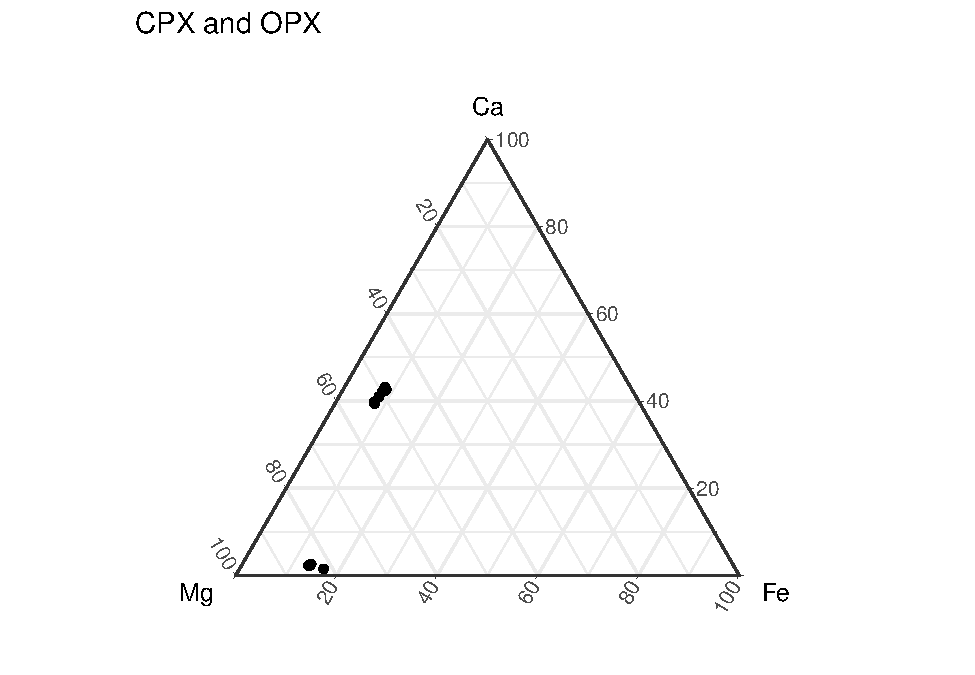
\includegraphics{KBH_94_23_DE_5_all_pyx_lines_files/figure-latex/unnamed-chunk-2-1.pdf}

\#OPX

\#Average Composition:

\begin{Shaded}
\begin{Highlighting}[]
\NormalTok{mol\_numbers }\OtherTok{\textless{}{-}} \FunctionTok{mutate}\NormalTok{(M5\_DE\_all\_OPX\_KBH\_94\_23, P2O5}\SpecialCharTok{/}\FloatTok{141.943}\NormalTok{,}\CommentTok{\#Change file here}
\NormalTok{                  SiO2}\SpecialCharTok{/}\FloatTok{53.083}\NormalTok{,}
\NormalTok{                  TiO2}\SpecialCharTok{/}\FloatTok{79.865}\NormalTok{,}
\NormalTok{                  Al2O3}\SpecialCharTok{/}\FloatTok{101.961}\NormalTok{,}
\NormalTok{                  Cr2O3}\SpecialCharTok{/}\FloatTok{99.993}\NormalTok{,}
\NormalTok{                  MgO}\SpecialCharTok{/}\FloatTok{40.304}\NormalTok{,}
\NormalTok{                  CaO}\SpecialCharTok{/}\FloatTok{56.077}\NormalTok{,}
\NormalTok{                  MnO}\SpecialCharTok{/}\FloatTok{70.937}\NormalTok{,}
\NormalTok{                  FeO}\SpecialCharTok{/}\FloatTok{71.844}\NormalTok{,}
\NormalTok{                  NiO}\SpecialCharTok{/}\FloatTok{74.692}\NormalTok{,}
\NormalTok{                  Na2O}\SpecialCharTok{/}\FloatTok{61.979}\NormalTok{,}
\NormalTok{                  K2O}\SpecialCharTok{/}\FloatTok{94.195}\NormalTok{)}

\NormalTok{oxygen\_number }\OtherTok{\textless{}{-}} \FunctionTok{mutate}\NormalTok{(mol\_numbers, }\AttributeTok{p =}\NormalTok{ P2O5}\SpecialCharTok{/}\FloatTok{141.943}\SpecialCharTok{*}\DecValTok{5}\NormalTok{,}
                        \AttributeTok{si =}\NormalTok{ SiO2}\SpecialCharTok{/}\FloatTok{53.083} \SpecialCharTok{*} \DecValTok{2}\NormalTok{,}
                        \AttributeTok{ti =}\NormalTok{ TiO2}\SpecialCharTok{/}\FloatTok{79.865} \SpecialCharTok{*} \DecValTok{2}\NormalTok{,}
                        \AttributeTok{al =}\NormalTok{ Al2O3}\SpecialCharTok{/}\FloatTok{101.961} \SpecialCharTok{*} \DecValTok{3}\NormalTok{,}
                        \AttributeTok{cr =}\NormalTok{ Cr2O3}\SpecialCharTok{/}\FloatTok{99.993} \SpecialCharTok{*} \DecValTok{3}\NormalTok{,}
                        \AttributeTok{mg =}\NormalTok{ MgO}\SpecialCharTok{/}\FloatTok{40.304} \SpecialCharTok{*} \DecValTok{1}\NormalTok{,}
                        \AttributeTok{ca =}\NormalTok{ CaO}\SpecialCharTok{/}\FloatTok{56.077} \SpecialCharTok{*} \DecValTok{1}\NormalTok{,}
                        \AttributeTok{mn =}\NormalTok{ MnO}\SpecialCharTok{/}\FloatTok{70.937} \SpecialCharTok{*} \DecValTok{1}\NormalTok{,}
                        \AttributeTok{fe =}\NormalTok{ FeO}\SpecialCharTok{/}\FloatTok{71.844} \SpecialCharTok{*} \DecValTok{1}\NormalTok{,}
                        \AttributeTok{ni =}\NormalTok{ NiO}\SpecialCharTok{/}\FloatTok{74.692} \SpecialCharTok{*} \DecValTok{1}\NormalTok{,}
                        \AttributeTok{na =}\NormalTok{ Na2O}\SpecialCharTok{/}\FloatTok{61.979} \SpecialCharTok{*} \DecValTok{1}\NormalTok{,}
                        \AttributeTok{k =}\NormalTok{ K2O}\SpecialCharTok{/}\FloatTok{94.195} \SpecialCharTok{*} \DecValTok{1}
\NormalTok{                        )}

\NormalTok{sum\_ox }\OtherTok{\textless{}{-}} \FunctionTok{select}\NormalTok{(oxygen\_number, p,}
\NormalTok{                   si,}
\NormalTok{                   ti,}
\NormalTok{                   al,}
\NormalTok{                   cr,}
\NormalTok{                   mg,}
\NormalTok{                   ca,}
\NormalTok{                   mn,}
\NormalTok{                   fe,}
\NormalTok{                   ni,}
\NormalTok{                   na,}
\NormalTok{                   k}
\NormalTok{                   )}

\NormalTok{sum\_row }\OtherTok{\textless{}{-}}\NormalTok{ sum\_ox }\SpecialCharTok{\%\textgreater{}\%} 
  \FunctionTok{mutate}\NormalTok{(}\AttributeTok{sum =} \FunctionTok{rowSums}\NormalTok{(.))}

\CommentTok{\#CHANGE BASED ON PYX=6 OL/SPI=4}

\NormalTok{six\_div\_sum }\OtherTok{\textless{}{-}} \FunctionTok{mutate}\NormalTok{(sum\_row,}\AttributeTok{norm\_constant =} \DecValTok{6}\SpecialCharTok{/}\NormalTok{sum) }\SpecialCharTok{\%\textgreater{}\%} 
  \FunctionTok{select}\NormalTok{(norm\_constant)}

\NormalTok{six\_div\_sum\_oxygen\_number }\OtherTok{\textless{}{-}} \FunctionTok{bind\_cols}\NormalTok{(oxygen\_number,six\_div\_sum)}

\NormalTok{oxy\_num\_mult\_norm\_const }\OtherTok{\textless{}{-}} \FunctionTok{mutate}\NormalTok{(six\_div\_sum\_oxygen\_number, }\AttributeTok{a =}\NormalTok{ p}\SpecialCharTok{*}\NormalTok{norm\_constant,}
                                  \AttributeTok{b =}\NormalTok{ si}\SpecialCharTok{*}\NormalTok{norm\_constant,}
                                  \AttributeTok{c =}\NormalTok{ ti}\SpecialCharTok{*}\NormalTok{norm\_constant,}
                                  \AttributeTok{d =}\NormalTok{ al}\SpecialCharTok{*}\NormalTok{norm\_constant,}
                                  \AttributeTok{e =}\NormalTok{ cr}\SpecialCharTok{*}\NormalTok{norm\_constant,}
                                  \AttributeTok{f =}\NormalTok{ mg}\SpecialCharTok{*}\NormalTok{norm\_constant,}
                                  \AttributeTok{g =}\NormalTok{ ca}\SpecialCharTok{*}\NormalTok{norm\_constant,}
                                  \AttributeTok{h =}\NormalTok{ mn}\SpecialCharTok{*}\NormalTok{norm\_constant,}
                                  \AttributeTok{i =}\NormalTok{ fe}\SpecialCharTok{*}\NormalTok{norm\_constant,}
                                  \AttributeTok{j =}\NormalTok{ ni}\SpecialCharTok{*}\NormalTok{norm\_constant,}
                                  \AttributeTok{k =}\NormalTok{ na}\SpecialCharTok{*}\NormalTok{norm\_constant,}
                                  \AttributeTok{l =}\NormalTok{ k}\SpecialCharTok{*}\NormalTok{norm\_constant}
\NormalTok{                                  )}

\NormalTok{mult\_cations }\OtherTok{\textless{}{-}} \FunctionTok{mutate}\NormalTok{(oxy\_num\_mult\_norm\_const, }\AttributeTok{a1 =}\NormalTok{ a }\SpecialCharTok{*} \DecValTok{2}\SpecialCharTok{/}\DecValTok{5}\NormalTok{,}
                       \AttributeTok{a2 =}\NormalTok{ b }\SpecialCharTok{*} \DecValTok{1}\SpecialCharTok{/}\DecValTok{2}\NormalTok{,}
                       \AttributeTok{a3 =}\NormalTok{ c }\SpecialCharTok{*} \DecValTok{1}\SpecialCharTok{/}\DecValTok{2}\NormalTok{,}
                       \AttributeTok{a4 =}\NormalTok{ d }\SpecialCharTok{*} \DecValTok{2}\SpecialCharTok{/}\DecValTok{3}\NormalTok{,}
                       \AttributeTok{a5 =}\NormalTok{ e }\SpecialCharTok{*} \DecValTok{2}\SpecialCharTok{/}\DecValTok{3}\NormalTok{,}
                       \AttributeTok{a6 =}\NormalTok{ f }\SpecialCharTok{*} \DecValTok{1}\SpecialCharTok{/}\DecValTok{1}\NormalTok{,}
                       \AttributeTok{a7 =}\NormalTok{ g }\SpecialCharTok{*} \DecValTok{1}\SpecialCharTok{/}\DecValTok{1}\NormalTok{,}
                       \AttributeTok{a8 =}\NormalTok{ h }\SpecialCharTok{*} \DecValTok{1}\SpecialCharTok{/}\DecValTok{1}\NormalTok{,}
                       \AttributeTok{a9 =}\NormalTok{ i }\SpecialCharTok{*} \DecValTok{1}\SpecialCharTok{/}\DecValTok{1}\NormalTok{,}
                       \AttributeTok{a10 =}\NormalTok{ j }\SpecialCharTok{*} \DecValTok{1}\SpecialCharTok{/}\DecValTok{1}\NormalTok{,}
                       \AttributeTok{a11 =}\NormalTok{ k }\SpecialCharTok{*} \DecValTok{2}\SpecialCharTok{/}\DecValTok{1}\NormalTok{,}
                       \AttributeTok{a12 =}\NormalTok{ l }\SpecialCharTok{*} \DecValTok{2}\SpecialCharTok{/}\DecValTok{1}\NormalTok{)}

\NormalTok{end }\OtherTok{\textless{}{-}}\NormalTok{ mult\_cations }\SpecialCharTok{\%\textgreater{}\%} 
  \FunctionTok{summarise}\NormalTok{(}\AttributeTok{ave\_P =} \FunctionTok{mean}\NormalTok{(a1),}
            \AttributeTok{ave\_Si =} \FunctionTok{mean}\NormalTok{(a2),}
            \AttributeTok{ave\_Ti =} \FunctionTok{mean}\NormalTok{(a3),}
            \AttributeTok{ave\_Al =} \FunctionTok{mean}\NormalTok{(a4),}
            \AttributeTok{ave\_Cr =} \FunctionTok{mean}\NormalTok{(a5),}
            \AttributeTok{ave\_Mg =} \FunctionTok{mean}\NormalTok{(a6),}
            \AttributeTok{ave\_Ca =} \FunctionTok{mean}\NormalTok{(a7),}
            \AttributeTok{ave\_Mn =} \FunctionTok{mean}\NormalTok{(a8),}
            \AttributeTok{ave\_Fe =} \FunctionTok{mean}\NormalTok{(a9),}
            \AttributeTok{ave\_Ni =} \FunctionTok{mean}\NormalTok{(a10),}
            \AttributeTok{ave\_Na =} \FunctionTok{mean}\NormalTok{(a11),}
            \AttributeTok{ave\_K =} \FunctionTok{mean}\NormalTok{(a12) }
\NormalTok{            )}
\NormalTok{show\_tbl\_2 }\OtherTok{\textless{}{-}}\NormalTok{ knitr}\SpecialCharTok{::}\FunctionTok{kable}\NormalTok{(end)}
\NormalTok{show\_tbl\_2}
\end{Highlighting}
\end{Shaded}

\begin{tabular}{r|r|r|r|r|r|r|r|r|r|r|r}
\hline
ave\_P & ave\_Si & ave\_Ti & ave\_Al & ave\_Cr & ave\_Mg & ave\_Ca & ave\_Mn & ave\_Fe & ave\_Ni & ave\_Na & ave\_K\\
\hline
0 & 1.938535 & 0.0055559 & 0.213224 & 0.0145782 & 1.481388 & 0.0398728 & 0.0049301 & 0.2397925 & 0 & 0.0080514 & 0.0155217\\
\hline
\end{tabular}

\hypertarget{ternary-for-opx-only}{%
\section{Ternary for OPX only}\label{ternary-for-opx-only}}

\begin{Shaded}
\begin{Highlighting}[]
\NormalTok{MgO\_num }\OtherTok{\textless{}{-}} \FunctionTok{mutate}\NormalTok{(M5\_DE\_all\_OPX\_KBH\_94\_23, }\AttributeTok{mg\_dat =}\NormalTok{ MgO}\SpecialCharTok{/}\FloatTok{40.304}\NormalTok{,}\CommentTok{\# Change file here too}
                  \AttributeTok{fe\_dat =}\NormalTok{ FeO}\SpecialCharTok{/}\FloatTok{71.844}\NormalTok{,}
                  \AttributeTok{ca\_dat =}\NormalTok{ CaO}\SpecialCharTok{/}\FloatTok{56.077}\NormalTok{,}
                  \AttributeTok{Mg =}\NormalTok{ (mg\_dat}\SpecialCharTok{/}\NormalTok{(mg\_dat}\SpecialCharTok{+}\NormalTok{fe\_dat}\SpecialCharTok{+}\NormalTok{ca\_dat))}\SpecialCharTok{*}\DecValTok{100}\NormalTok{,}
                  \AttributeTok{Fe =}\NormalTok{ (fe\_dat}\SpecialCharTok{/}\NormalTok{(mg\_dat}\SpecialCharTok{+}\NormalTok{fe\_dat}\SpecialCharTok{+}\NormalTok{ca\_dat))}\SpecialCharTok{*}\DecValTok{100}\NormalTok{,}
                  \AttributeTok{Ca =}\NormalTok{ (ca\_dat}\SpecialCharTok{/}\NormalTok{(mg\_dat}\SpecialCharTok{+}\NormalTok{fe\_dat}\SpecialCharTok{+}\NormalTok{ca\_dat))}\SpecialCharTok{*}\DecValTok{100}
\NormalTok{                  ) }

\NormalTok{  tern }\OtherTok{\textless{}{-}} \FunctionTok{ggtern}\NormalTok{(}\AttributeTok{data =}\NormalTok{ MgO\_num, }\FunctionTok{aes}\NormalTok{(}\AttributeTok{x =}\NormalTok{ Mg,}
                          \AttributeTok{y =}\NormalTok{ Ca, }
                          \AttributeTok{z =}\NormalTok{ Fe)) }\SpecialCharTok{+}
  \FunctionTok{geom\_point}\NormalTok{()}\SpecialCharTok{+}
    \FunctionTok{labs}\NormalTok{(}\AttributeTok{title =} \StringTok{"OPX"}\NormalTok{)}\SpecialCharTok{+}
    \FunctionTok{theme\_bw}\NormalTok{()}
  
\NormalTok{  tern}
\end{Highlighting}
\end{Shaded}

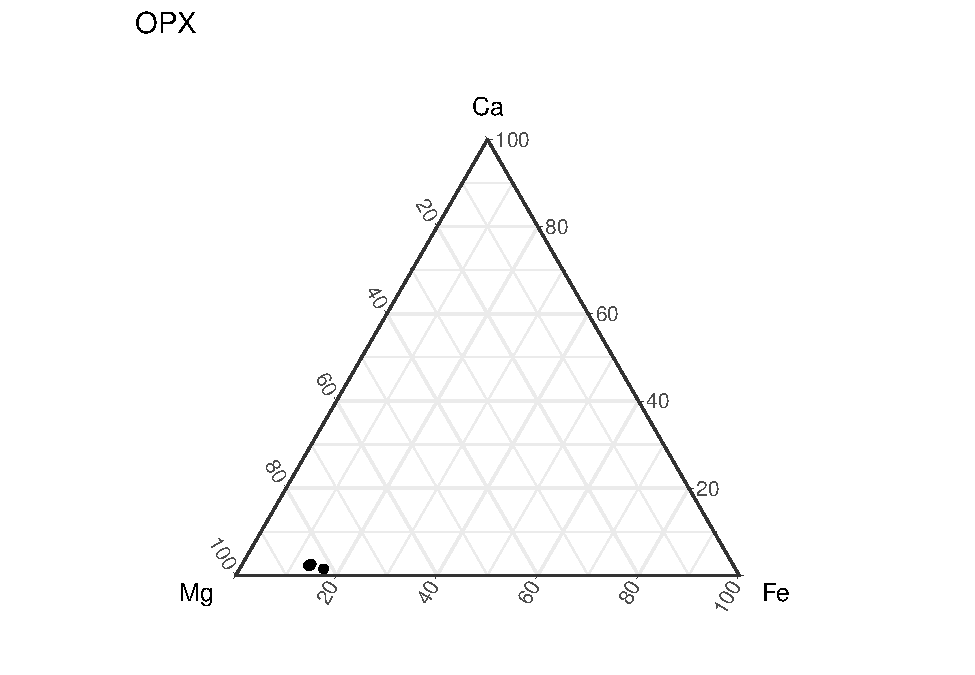
\includegraphics{KBH_94_23_DE_5_all_pyx_lines_files/figure-latex/unnamed-chunk-5-1.pdf}

\#CPX

\#Ave composition of CPX

\begin{Shaded}
\begin{Highlighting}[]
\NormalTok{mol\_numbers }\OtherTok{\textless{}{-}} \FunctionTok{mutate}\NormalTok{(M5\_DE\_all\_CPX\_KBH\_94\_23, P2O5}\SpecialCharTok{/}\FloatTok{141.943}\NormalTok{,}\CommentTok{\#Change file here}
\NormalTok{                  SiO2}\SpecialCharTok{/}\FloatTok{53.083}\NormalTok{,}
\NormalTok{                  TiO2}\SpecialCharTok{/}\FloatTok{79.865}\NormalTok{,}
\NormalTok{                  Al2O3}\SpecialCharTok{/}\FloatTok{101.961}\NormalTok{,}
\NormalTok{                  Cr2O3}\SpecialCharTok{/}\FloatTok{99.993}\NormalTok{,}
\NormalTok{                  MgO}\SpecialCharTok{/}\FloatTok{40.304}\NormalTok{,}
\NormalTok{                  CaO}\SpecialCharTok{/}\FloatTok{56.077}\NormalTok{,}
\NormalTok{                  MnO}\SpecialCharTok{/}\FloatTok{70.937}\NormalTok{,}
\NormalTok{                  FeO}\SpecialCharTok{/}\FloatTok{71.844}\NormalTok{,}
\NormalTok{                  NiO}\SpecialCharTok{/}\FloatTok{74.692}\NormalTok{,}
\NormalTok{                  Na2O}\SpecialCharTok{/}\FloatTok{61.979}\NormalTok{,}
\NormalTok{                  K2O}\SpecialCharTok{/}\FloatTok{94.195}\NormalTok{)}

\NormalTok{oxygen\_number }\OtherTok{\textless{}{-}} \FunctionTok{mutate}\NormalTok{(mol\_numbers, }\AttributeTok{p =}\NormalTok{ P2O5}\SpecialCharTok{/}\FloatTok{141.943}\SpecialCharTok{*}\DecValTok{5}\NormalTok{,}
                        \AttributeTok{si =}\NormalTok{ SiO2}\SpecialCharTok{/}\FloatTok{53.083} \SpecialCharTok{*} \DecValTok{2}\NormalTok{,}
                        \AttributeTok{ti =}\NormalTok{ TiO2}\SpecialCharTok{/}\FloatTok{79.865} \SpecialCharTok{*} \DecValTok{2}\NormalTok{,}
                        \AttributeTok{al =}\NormalTok{ Al2O3}\SpecialCharTok{/}\FloatTok{101.961} \SpecialCharTok{*} \DecValTok{3}\NormalTok{,}
                        \AttributeTok{cr =}\NormalTok{ Cr2O3}\SpecialCharTok{/}\FloatTok{99.993} \SpecialCharTok{*} \DecValTok{3}\NormalTok{,}
                        \AttributeTok{mg =}\NormalTok{ MgO}\SpecialCharTok{/}\FloatTok{40.304} \SpecialCharTok{*} \DecValTok{1}\NormalTok{,}
                        \AttributeTok{ca =}\NormalTok{ CaO}\SpecialCharTok{/}\FloatTok{56.077} \SpecialCharTok{*} \DecValTok{1}\NormalTok{,}
                        \AttributeTok{mn =}\NormalTok{ MnO}\SpecialCharTok{/}\FloatTok{70.937} \SpecialCharTok{*} \DecValTok{1}\NormalTok{,}
                        \AttributeTok{fe =}\NormalTok{ FeO}\SpecialCharTok{/}\FloatTok{71.844} \SpecialCharTok{*} \DecValTok{1}\NormalTok{,}
                        \AttributeTok{ni =}\NormalTok{ NiO}\SpecialCharTok{/}\FloatTok{74.692} \SpecialCharTok{*} \DecValTok{1}\NormalTok{,}
                        \AttributeTok{na =}\NormalTok{ Na2O}\SpecialCharTok{/}\FloatTok{61.979} \SpecialCharTok{*} \DecValTok{1}\NormalTok{,}
                        \AttributeTok{k =}\NormalTok{ K2O}\SpecialCharTok{/}\FloatTok{94.195} \SpecialCharTok{*} \DecValTok{1}
\NormalTok{                        )}

\NormalTok{sum\_ox }\OtherTok{\textless{}{-}} \FunctionTok{select}\NormalTok{(oxygen\_number, p,}
\NormalTok{                   si,}
\NormalTok{                   ti,}
\NormalTok{                   al,}
\NormalTok{                   cr,}
\NormalTok{                   mg,}
\NormalTok{                   ca,}
\NormalTok{                   mn,}
\NormalTok{                   fe,}
\NormalTok{                   ni,}
\NormalTok{                   na,}
\NormalTok{                   k}
\NormalTok{                   )}

\NormalTok{sum\_row }\OtherTok{\textless{}{-}}\NormalTok{ sum\_ox }\SpecialCharTok{\%\textgreater{}\%} 
  \FunctionTok{mutate}\NormalTok{(}\AttributeTok{sum =} \FunctionTok{rowSums}\NormalTok{(.))}

\CommentTok{\#CHANGE BASED ON PYX=6 OL/SPI=4}

\NormalTok{six\_div\_sum }\OtherTok{\textless{}{-}} \FunctionTok{mutate}\NormalTok{(sum\_row,}\AttributeTok{norm\_constant =} \DecValTok{6}\SpecialCharTok{/}\NormalTok{sum) }\SpecialCharTok{\%\textgreater{}\%} 
  \FunctionTok{select}\NormalTok{(norm\_constant)}

\NormalTok{six\_div\_sum\_oxygen\_number }\OtherTok{\textless{}{-}} \FunctionTok{bind\_cols}\NormalTok{(oxygen\_number,six\_div\_sum)}

\NormalTok{oxy\_num\_mult\_norm\_const }\OtherTok{\textless{}{-}} \FunctionTok{mutate}\NormalTok{(six\_div\_sum\_oxygen\_number, }\AttributeTok{a =}\NormalTok{ p}\SpecialCharTok{*}\NormalTok{norm\_constant,}
                                  \AttributeTok{b =}\NormalTok{ si}\SpecialCharTok{*}\NormalTok{norm\_constant,}
                                  \AttributeTok{c =}\NormalTok{ ti}\SpecialCharTok{*}\NormalTok{norm\_constant,}
                                  \AttributeTok{d =}\NormalTok{ al}\SpecialCharTok{*}\NormalTok{norm\_constant,}
                                  \AttributeTok{e =}\NormalTok{ cr}\SpecialCharTok{*}\NormalTok{norm\_constant,}
                                  \AttributeTok{f =}\NormalTok{ mg}\SpecialCharTok{*}\NormalTok{norm\_constant,}
                                  \AttributeTok{g =}\NormalTok{ ca}\SpecialCharTok{*}\NormalTok{norm\_constant,}
                                  \AttributeTok{h =}\NormalTok{ mn}\SpecialCharTok{*}\NormalTok{norm\_constant,}
                                  \AttributeTok{i =}\NormalTok{ fe}\SpecialCharTok{*}\NormalTok{norm\_constant,}
                                  \AttributeTok{j =}\NormalTok{ ni}\SpecialCharTok{*}\NormalTok{norm\_constant,}
                                  \AttributeTok{k =}\NormalTok{ na}\SpecialCharTok{*}\NormalTok{norm\_constant,}
                                  \AttributeTok{l =}\NormalTok{ k}\SpecialCharTok{*}\NormalTok{norm\_constant}
\NormalTok{                                  )}

\NormalTok{mult\_cations }\OtherTok{\textless{}{-}} \FunctionTok{mutate}\NormalTok{(oxy\_num\_mult\_norm\_const, }\AttributeTok{a1 =}\NormalTok{ a }\SpecialCharTok{*} \DecValTok{2}\SpecialCharTok{/}\DecValTok{5}\NormalTok{,}
                       \AttributeTok{a2 =}\NormalTok{ b }\SpecialCharTok{*} \DecValTok{1}\SpecialCharTok{/}\DecValTok{2}\NormalTok{,}
                       \AttributeTok{a3 =}\NormalTok{ c }\SpecialCharTok{*} \DecValTok{1}\SpecialCharTok{/}\DecValTok{2}\NormalTok{,}
                       \AttributeTok{a4 =}\NormalTok{ d }\SpecialCharTok{*} \DecValTok{2}\SpecialCharTok{/}\DecValTok{3}\NormalTok{,}
                       \AttributeTok{a5 =}\NormalTok{ e }\SpecialCharTok{*} \DecValTok{2}\SpecialCharTok{/}\DecValTok{3}\NormalTok{,}
                       \AttributeTok{a6 =}\NormalTok{ f }\SpecialCharTok{*} \DecValTok{1}\SpecialCharTok{/}\DecValTok{1}\NormalTok{,}
                       \AttributeTok{a7 =}\NormalTok{ g }\SpecialCharTok{*} \DecValTok{1}\SpecialCharTok{/}\DecValTok{1}\NormalTok{,}
                       \AttributeTok{a8 =}\NormalTok{ h }\SpecialCharTok{*} \DecValTok{1}\SpecialCharTok{/}\DecValTok{1}\NormalTok{,}
                       \AttributeTok{a9 =}\NormalTok{ i }\SpecialCharTok{*} \DecValTok{1}\SpecialCharTok{/}\DecValTok{1}\NormalTok{,}
                       \AttributeTok{a10 =}\NormalTok{ j }\SpecialCharTok{*} \DecValTok{1}\SpecialCharTok{/}\DecValTok{1}\NormalTok{,}
                       \AttributeTok{a11 =}\NormalTok{ k }\SpecialCharTok{*} \DecValTok{2}\SpecialCharTok{/}\DecValTok{1}\NormalTok{,}
                       \AttributeTok{a12 =}\NormalTok{ l }\SpecialCharTok{*} \DecValTok{2}\SpecialCharTok{/}\DecValTok{1}\NormalTok{)}

\NormalTok{end }\OtherTok{\textless{}{-}}\NormalTok{ mult\_cations }\SpecialCharTok{\%\textgreater{}\%} 
  \FunctionTok{summarise}\NormalTok{(}\AttributeTok{ave\_P =} \FunctionTok{mean}\NormalTok{(a1),}
            \AttributeTok{ave\_Si =} \FunctionTok{mean}\NormalTok{(a2),}
            \AttributeTok{ave\_Ti =} \FunctionTok{mean}\NormalTok{(a3),}
            \AttributeTok{ave\_Al =} \FunctionTok{mean}\NormalTok{(a4),}
            \AttributeTok{ave\_Cr =} \FunctionTok{mean}\NormalTok{(a5),}
            \AttributeTok{ave\_Mg =} \FunctionTok{mean}\NormalTok{(a6),}
            \AttributeTok{ave\_Ca =} \FunctionTok{mean}\NormalTok{(a7),}
            \AttributeTok{ave\_Mn =} \FunctionTok{mean}\NormalTok{(a8),}
            \AttributeTok{ave\_Fe =} \FunctionTok{mean}\NormalTok{(a9),}
            \AttributeTok{ave\_Ni =} \FunctionTok{mean}\NormalTok{(a10),}
            \AttributeTok{ave\_Na =} \FunctionTok{mean}\NormalTok{(a11),}
            \AttributeTok{ave\_K =} \FunctionTok{mean}\NormalTok{(a12) }
\NormalTok{            )}

\NormalTok{show\_tbl\_3 }\OtherTok{\textless{}{-}}\NormalTok{ knitr}\SpecialCharTok{::}\FunctionTok{kable}\NormalTok{(end)}
\NormalTok{show\_tbl\_3}
\end{Highlighting}
\end{Shaded}

\begin{tabular}{r|r|r|r|r|r|r|r|r|r|r|r}
\hline
ave\_P & ave\_Si & ave\_Ti & ave\_Al & ave\_Cr & ave\_Mg & ave\_Ca & ave\_Mn & ave\_Fe & ave\_Ni & ave\_Na & ave\_K\\
\hline
0 & 1.920044 & 0.0161248 & 0.2937758 & 0.0318024 & 0.7901361 & 0.6697853 & 0.0034842 & 0.1302866 & 0 & 0.0909568 & 0.1808839\\
\hline
\end{tabular}

\hypertarget{ternary-of-cpx-only}{%
\section{Ternary of CPX only}\label{ternary-of-cpx-only}}

\begin{Shaded}
\begin{Highlighting}[]
\NormalTok{MgO\_num }\OtherTok{\textless{}{-}} \FunctionTok{mutate}\NormalTok{(M5\_DE\_all\_CPX\_KBH\_94\_23, }\AttributeTok{mg\_dat =}\NormalTok{ MgO}\SpecialCharTok{/}\FloatTok{40.304}\NormalTok{,}\CommentTok{\# Change file here too}
                  \AttributeTok{fe\_dat =}\NormalTok{ FeO}\SpecialCharTok{/}\FloatTok{71.844}\NormalTok{,}
                  \AttributeTok{ca\_dat =}\NormalTok{ CaO}\SpecialCharTok{/}\FloatTok{56.077}\NormalTok{,}
                  \AttributeTok{Mg =}\NormalTok{ (mg\_dat}\SpecialCharTok{/}\NormalTok{(mg\_dat}\SpecialCharTok{+}\NormalTok{fe\_dat}\SpecialCharTok{+}\NormalTok{ca\_dat))}\SpecialCharTok{*}\DecValTok{100}\NormalTok{,}
                  \AttributeTok{Fe =}\NormalTok{ (fe\_dat}\SpecialCharTok{/}\NormalTok{(mg\_dat}\SpecialCharTok{+}\NormalTok{fe\_dat}\SpecialCharTok{+}\NormalTok{ca\_dat))}\SpecialCharTok{*}\DecValTok{100}\NormalTok{,}
                  \AttributeTok{Ca =}\NormalTok{ (ca\_dat}\SpecialCharTok{/}\NormalTok{(mg\_dat}\SpecialCharTok{+}\NormalTok{fe\_dat}\SpecialCharTok{+}\NormalTok{ca\_dat))}\SpecialCharTok{*}\DecValTok{100}
\NormalTok{                  ) }

\NormalTok{  tern }\OtherTok{\textless{}{-}} \FunctionTok{ggtern}\NormalTok{(}\AttributeTok{data =}\NormalTok{ MgO\_num, }\FunctionTok{aes}\NormalTok{(}\AttributeTok{x =}\NormalTok{ Mg,}
                          \AttributeTok{y =}\NormalTok{ Ca, }
                          \AttributeTok{z =}\NormalTok{ Fe)) }\SpecialCharTok{+}
  \FunctionTok{geom\_point}\NormalTok{()}\SpecialCharTok{+}
    \FunctionTok{labs}\NormalTok{(}\AttributeTok{title =} \StringTok{"CPX"}\NormalTok{)}\SpecialCharTok{+}
    \FunctionTok{theme\_bw}\NormalTok{()}
  
\NormalTok{  tern}
\end{Highlighting}
\end{Shaded}

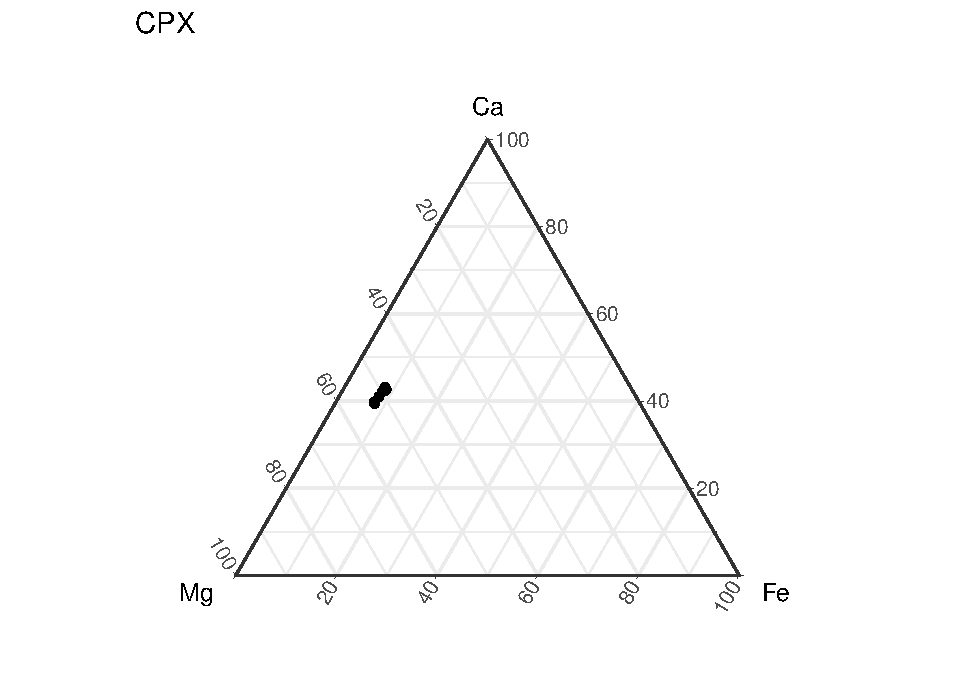
\includegraphics{KBH_94_23_DE_5_all_pyx_lines_files/figure-latex/unnamed-chunk-8-1.pdf}

\end{document}
